\documentclass[11pt,a4paper, notitlepage]{article}

% --- Packages ---
\usepackage[utf8]{inputenc}
\usepackage{geometry}
\geometry{margin=1in}
\usepackage{graphicx}
\usepackage{amsmath} 
\usepackage{listings} 
\usepackage{xurl}
\usepackage[hidelinks]{hyperref}
\usepackage{titlesec}
\usepackage{titling}
\usepackage{float}
\setlength{\droptitle}{-2cm}
\hypersetup{breaklinks=true}

% --- Document Info ---
\title{Detecting Cache Side-Channel Attacks in Multi-tenant OpenShift Environments}
\author{Sami Bensalah}
\date{\today}

\begin{document}

\maketitle
\begin{abstract}
\footnotesize
This report describes the design, implementation and deployment of a cache side-channel attack detection service on a Red Hat OpenShift (RHOCP) cluster and investigates its effectiveness for defending against cross-tenant cloud attacks. I describe the development and effectiveness of a Prime+Probe attack on the LLC enabled by a spectre v1 (bounds check bypass) side-channel vulnerability in a targeted victim server and outline an implementation for a system to reliably and accurately detecting these attacks based on microarchitectural telemetry.
\end{abstract}



\section{Introduction}
\subsection{Motivation}
\subsubsection{Public Cloud Vulnerability}
While OpenShift and all host cloud platforms provide logical isolation and hardware virtualisation, the underlying CPU cache remains a shared resource across all processes. Many cloud platforms are able to offer significantly cheaper cloud infrastructure by partitioning a single powerful server into various logically seperated tenant spaces, creating a multi-tenant cloud environment. This method of divying out server resources gave rise to the public cloud architecture used by the majority of enterprises, and though cloud security concerns for public cloud has been raised leading to the now wider application of hybrid cloud some businesses still have vulnerable services running on environments susceptible to cross-tenant cloud attacks.
\subsubsection{Mitigation Effectiveness and Performance}
The discovery of spectre and meltdown attacks in 2018 and subsequent attacks resulted in CPU manufacturers and OS distributors scrambling to introduce mitigations through software patches and hardware-level blocks. Though the ability for meltdown to function has been practically removed by these mitigations, spectre variants still pose a serious risk. The main reason for this being that speculative execution is an inherent part of modern CPU architecture, removing speculation would reduce CPU throughput drastically. 

Variants of spectre require different targeted mitigations which makes them so hard to prevent, particularly spectre v1 bounds check bypass. They have various linux kernel level mitigations currently available, such as Indirect Branch Prediction Barrier (IBPB), Single Thread Indirect Branch Predictors (STIBP) and LFENCE (v1 specific). However, as outlined in the Linux kernel documentation `the protections are put in place on a case by case basis, and there is no guarantee that all possible attack vectors for spectre variant 1 are covered'~\cite{kernel_spectre}. In the case of spectre v1, the main mitigation strategy is defensive programming and inserting LFENCEs before vulnerable branches, however, in certain constrained systems constant instruction fences are not feasible, leading to extremely vulnerable processes being in production. 

This performance degradation was also noted by Red Hat with their own kernel patches where they mentioned ``Speculative execution is a performance optimization technique which these updates change (both kernel and microcode) and may result in workload-specific performance degradation."~\cite{redhat2019}. Despite Red Hat having these denfenses enabled by default, the performance penalty is severe enough that Red Hat and the Linux kernel provide mechanisms to bypass these protections. Resulting in various insecure environments possibly running with no mitigations enabled in the cloud.

\subsubsection{OpenShift Clusters}
OpenShift clusters are an industry standard method of deploying applications onto cloud infrastructure securely and effectively, with ``50\% of the top Fortune 100 companies are using Red Hat OpenShift" \cite{openshift_usage}. This huge client base results in a large number of services running on these clusters, and in very few cases are the clusters not hosted on a type of cloud infrastructure. As discussed previously, this leads to the possibility of being a target of a side-channel attack.

\subsection{Problem Definition}
My motivation leads me to my goal for this project, which is to detect if a cache side-channel has occurred on any monitored service within the RHOCP cluster. The objective is to remove the need to decide between prioritising performance over security and allow a more globally usable mitigation strategy independent of the underlying environment architecture. So, rather than having to employ hard counters to the attacks, such as the software and hardware mitigations for spectre available, we instead employ a soft mitigation strategy, which involves a sophisticated detector sending a trustable signal if an attack is occuring live, to facilitate the triggering of defensive actions, such as moving a service onto a different cluster node running on a seperate physical machine or killing the container. 

\begin{center}
\rule{0.8\textwidth}{0.4pt} \\ \vspace{0.2cm}
\begin{minipage}{0.8\textwidth}
\small \textbf{NOTE:} the report does not discuss how to implement defensive actions but focuses on the system designed to detect the presence of these attacks on running cluster workloads. The mitigation strategies needed post detection would very by use-case and would need to be carefully thought through by the implementor.
\end{minipage} \\ \vspace{0.2cm}
\rule{0.8\textwidth}{0.4pt}
\end{center}

\section{Project Background}
\subsection{Cache Structure and Mapping}
\label{sec:cache_structure}
Cache is structured with levels, most commonly with a 3 level cache design which is made up of L1, L2 and L3/LLC (Last Level Cache).
In many ARM systems, you can have distinct instruction and data level 1 caches backed by a 'unified' level for L2 and L3~\cite{arm_architecture}.
Each cache level consists of sets, ways and lines. A set defines a region of cache where memory addresses will map to based on the value of the address' index bits, as highlighted in Figure \ref{fig:cache_mapping}.
\begin{figure}[H] 
    \centering
    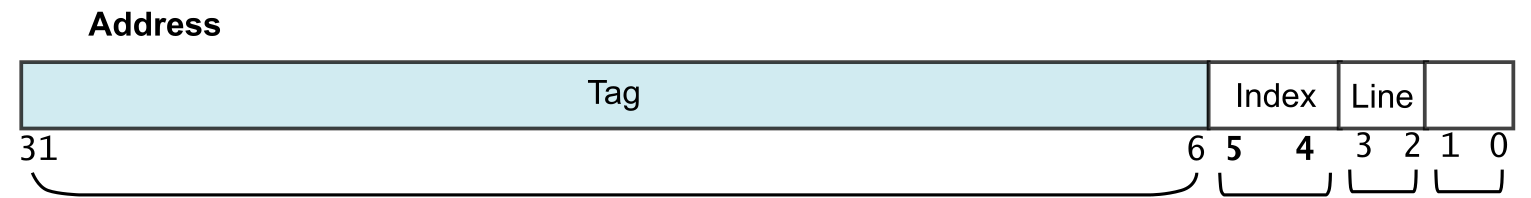
\includegraphics[width=0.7\textwidth]{images/memaddr_format.png}
    \caption{Tag, Index, and Offset bits of a physical memory address for cache mapping \cite{arm_architecture}}
    \label{fig:cache_mapping}
\end{figure}
Associativity defines the number of ways (individual cache lines) within a set and a cache line (64 bytes) refers to a `cell' or space within the set that a memory address store its data.
Associativity changes depending on the overall system and level cache. Higher levels of cache often have higher associativity resulting in more lines within the set and a higher cache capacity as seen in Table \ref{tab:cache_specs_grid}.  
\begin{table}[!htbp]
\centering
\caption{Microarchitectural cache specifications of the lab cluster node.}
\label{tab:cache_specs_grid}
\begin{tabular}{|l|l|l|l|l|}
\hline
\textbf{Cache Level} & \textbf{Size} & \textbf{Associativity} & \textbf{Sets} & \textbf{Type} \\ \hline
L1 Data (L1d)        & 32 KB         & 8-way                  & 64            & Private       \\ \hline
L1 Instruction (L1i) & 32 KB         & 8-way                  & 64            & Private       \\ \hline
L2 Cache             & 256 KB       & 16-way                 & 1024          & Private       \\ \hline
L3 Cache (LLC)       & 12 MB         & 24-way                 & 12288         & Shared        \\ \hline
\end{tabular}
\end{table}

Another term which will be referenced is cache stride (or set stride), which refers to the number of indexes within a byte array which correspond to memory addresses that map to the same set (i.e., have the same index bits). It is often the size of a page of memory (4096 bytes for standard pages) but is dependent on the data type of the array/list. Its primary function for an attacker which will be discussed further is to build eviction sets (a collection of addresses which can `take over' a cache set).


\subsection{Spectre V1 (Bounds Check Bypass)}
Spectre V1 is an attack that targets and exploits conditional branches; ``the attacker mistrains the CPU’s branch predictor into mispredicting the direction of a branch, causing the CPU to temporarily violate program semantics by executing code that would not have been executed otherwise'' \cite{spectre_og}.
This act of training the branch predictor can also be referred to as poisoning, and within modern CPUs, there are two primary mechanisms for branch prediction: global and local.
The global branch predictor uses a more holistic approach and infers the relationships between branches based on prior executions to predict the branch's outcome. 
In contrast, local branch predictors look at each branch instruction individually and base their prediction independent of the rest of the program's execution. This localized mechanism is the target used in this study. 

So, although the architectural state is rolled back when the CPU realises its misprediction, a `ghost' signal or `footprint' is left behind in cache. The code within the branch known as a spectre `gadget' is in place within the victim's vulnerable branchh which is executed post transient execution resulting in a cache mapping which the adversary can predict and infer a set of values from.
\subsection{Cache Timing Side-Channels}
A side channel attack is any unintended side effect which can be measured to infer information during a program's execution. In this report I will be discussing side-channel timing attacks specifically which are enabled by the spectre v1 gadget.
The timing attacks I used are Prime+Probe and Flush+Reload. 
\subsubsection{Flush+Reload}
Flush+Reload is a widely used attack with the majority of research papers on spectre employ Flush+Reload as a mechanism to read the cache residue caused by the transient execution.
It involves flushing a target address' data from memory, spectre v1 is then triggered and if the spectre gadget maps to that flushed address it speculatively accesses it. We then perform the reload which is where we measure our timing side-channel, 
this involves measuring the fetch time using hardware level timers. If the fetch time is under a certain cycle threshold then we can infer that the address, though it was previously flushed, is now in cache, meaning that it was used speculatively, allowing us to infer and steal secret information.

The issue in applying this attack to cloud systems for cross-tenant attacks is that the adversary requires access to the same memory space to be able to flush, making this attack infeasible on virtualised and logically isolated user spaces. 

\subsubsection{Prime+Probe on L1 and Last Level Cache LLC}
Prime+Probe is a significantly more sophisticated approach in comparison to Flush+Reload as, rather than relying on access to a shared memory space, it instead requires a shared environment on the hardware level only.
This results in a much more effective method for cross-VM attacks on multi-tenant environments, hence why it has been chosen as the main approach for this project. 

Prime+Probe begins with the priming phase, which involves creating an eviction set targeting a specific cache set (Step 1 of Figure \ref{fig:prime_probe}), as discussed in Section \ref{sec:cache_structure}. This noramlly involves requesting a large portion of memory by creating a large array of several megabytes and picking out useful memory addresses to use in the attack. 
The spectre gadget will then be triggered causing the victim to touch the cache and evict an address from the eviction set (Step 2 of Figure \ref{fig:prime_probe}). During the prime phase the attacker fetches and times each addresses to see if there have been any evictions (i.e., has the attacker data has been forced out of cache by victim activity).
If an address has been evicted then that is classified as a `cache miss' (Step 3 of Figure \ref{fig:prime_probe}) and if it is fetched in expected time (i.e., it was still in cache during probe) then it is classified as a `cache hit'. 

\begin{figure}[H] 
    \centering
    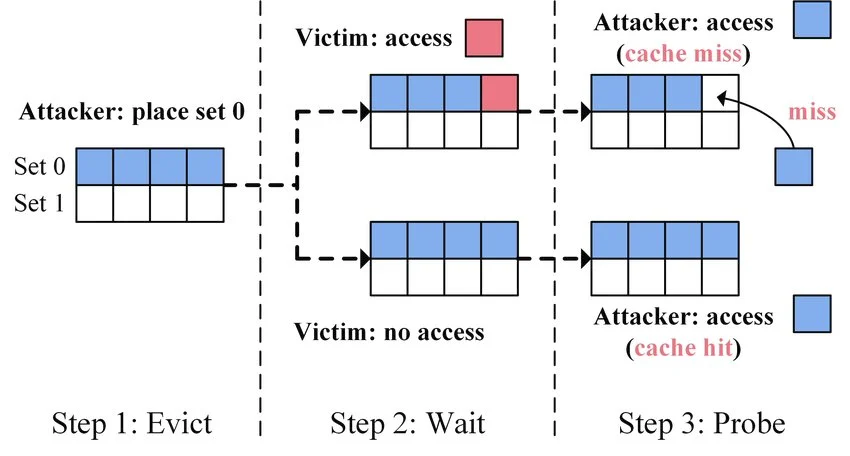
\includegraphics[width=0.7\textwidth]{images/prime_probe.png}
    \caption{Prime + Probe cache attacks. The timing difference (cache hits or cache misses) discloses the victim's access pattern. \cite{prime_probe_img}}
    \label{fig:prime_probe}
\end{figure}

Cache is inherently noisy and evictions are constantly occurring leading to various misses during system runtime. This also means that the attack will result in various false misses, where the probe phase identifies that an address' data has been replaced, in a quiet system it is most likely due to the victim, however,
in noisier multi-tenant cloud systems noise will be introduced by a third party, such as other users, kernel activities or other cluster services. This makes Prime+Probe less reliable on noisier systems which in most cases is fixed by increasing the number of repeat runs by 10s of thousands to ensre that the cache signal is true.


\subsection{OpenShift}
\subsection{PMU and Hardware Counters}

\section{Methodology}
\subsection{Attack Framework}
\subsection{Detection Logic and Threshold Analysis}

\section{Implementation}
\subsection{Detection Service}
\subsection{Spectre Gadget}
\subsubsection{Flush+Reload Validation}
\subsection{Prime+Probe Implementation}
\subsubsection{L1 Targeting}
\subsubsection{Last Level Cache Targeting}


\begin{thebibliography}{9}

\bibitem{kernel_spectre}
Linux Kernel Organization, 
``Spectre Side Channels,'' 
\emph{The Linux Kernel Administration Guide}, 2024. [Online]. Available: \url{https://docs.kernel.org/admin-guide/hw-vuln/spectre.html}

\bibitem{redhat2019}
Red Hat Customer Portal, 
``Controlling the Impact of Speculative Execution Vulnerabilities,'' 
2020. [Online]. Available: \url{https://access.redhat.com/articles/3311301}

\bibitem{openshift_usage}
Red Hat, 
``More Than 1,000 Enterprises Across the Globe Adopt Red Hat OpenShift Container Platform to Power Business Applications'' 
2019. [Online]. Available: \url{https://www.redhat.com/en/about/press-releases/more-1000-enterprises-across-globe-adopt-red-hat-openshift-container-platform-power-business-applications}

\bibitem{arm_architecture}
Arm Limited, 
``Cache Architecture,'' 
\emph{Arm Cortex-A Series Programmer's Guide}, 2026. [Online]. Available: \url{https://developer.arm.com/documentation/den0013/0400/Caches/Cache-architecture}

\bibitem{spectre_og}
Spectre Attack, 
``Spectre Attacks: Exploiting Speculative Execution'' 
\emph{Spectre Attacks: Exploiting Speculative Execution}. [Online]. Available: \url{https://spectreattack.com/spectre.pdf}

\bibitem{primeprobe}
IEEE Symposium on Security and Privacy, 
``Last-Level Cache Side-Channel Attacks are Practical'' 
\emph{Last-Level Cache Side-Channel Attacks are Practical}, 2015. [Online]. Available: \url{https://www.cse.iitb.ac.in/~biswa/courses/CS773/lectures/primeprobe.pdf}

\bibitem{prime_probe_img}
K.~Wang, F.~Yuan, L.~Zhao, and D.~Meng, 
``Secure hybrid replacement policy: Mitigating conflict-based cache side channel attacks,'' 
\textit{ResearchGate [Scientific Figure]}, Jan. 2022. 
Available: \url{https://www.researchgate.net/figure/Prime-Probe-cache-attacks-The-timing-difference-cache-hits-or-cache-misses-discloses_fig1_357728625} [Accessed 22-Mar-2026].

\end{thebibliography}

\end{document}